\chapter{Horizontale Evolution} % 8 Seiten

Im Fokus dieses Kapitel steht die Einführung von agilen Vorgehensmodellen in sicherheitskritischen Bereichen.
Damit die Unterschiede gegenüber den klassischen Bereichen ersichtlich werden, folgt zuerst eine Untersuchung der Vorgehensmodelle in klassischen Bereichen.
Bei den sicherheitskritischen Bereiche wird insbesondere auf die Luft- und Raumfahrtindustrie (NASA, ESA, etc.) eingegangen.

\section{Agile Vorgehensmodelle in klassischen Bereichen} % 4 Seiten 

Nachfolgend wird auf die Auswirkungen von agilen Vorgehensmodellen, die Herausforderungen, Vor- und Nachteile in klassischen Bereichen eingegangen.
Dazu werden mehrere Fallstudien analysiert.

\subsection{Kommunikation} % 1 Seite

Durch die Einführung von agilen Prozessen wird auch die Entscheidungsfindung in Unternehmen stark verändert.
Dabei wird von einem Führungsmodell mit starken Autorität zu einem verteilten, selbst organisierenden Modell gewechselt.
Involviert sind die einzelnen Entwicklerteams sowie externe Stakeholder.
Es wird ein Kommunikationskonzept umgesetzt, welches den autoritäten Teil so weit wie möglich verringert.
Dies ist jedoch ein wesentlich komplexeres Modell, da die Entscheidungsfindung nun nicht mehr nur bei einer einzelnen Person, dem Manager, sondern bei jedem Teammitglied liegt.
Während in klassischen Vorgehensmodellen klare Vorgaben an die Teammitglieder gestellt werden, müssen diese in agilen Modellen auch Verantwortung für das Controlling ihrer eigenen Leistung übernehmen.
Dadurch wird auch implizit die Verantwortung einer Entscheidung jeweils an die Person verlagert, die das relevante Wissen bezüglich dieser Entscheidung besitzt.
Dies hat zur Folge, dass der klassische Projektmanager sich auf die reinen Verwaltungsaufgaben konzentrieren kann und sich nicht in fachliche Details einarbeiten muss.
Durch die Verlagerung der Entscheidung an näher am Problem liegende Stellen wird eine Verbesserung in der Lösung des Problems bezüglich Geschwindigkeit und Qualität erreicht.
Zur Umsetzung dieser selbst organisierenden Teams muss jedoch mehr umgesetzt werden, als nur flache Hierarchien und demokratische Prozesse zu implementieren.
Dabei sind folgende Maßnahmen als effektiv eingestuft:
\begin{itemize}
\item Klare Ausrichtung der Teams
\item Eine leistungsfördernde Teamstruktur
\item Ein untersützender organisatorischer Kontext
\item Coaching durch einen Experten
\item Vorhandene und passende Ressourcen
\end{itemize}
\parencite[Vgl.][S. 863 f.]{Moe:2012aa}

Da kleine, selbst organisierende Teams Personen nahe zueinander bringen, haben diese auch einen positiven Einfluss auf die generelle Kommunikation zwischen den Teammitgliedern.
Zusätzlich kann anfallende Dokumentation minimiert werden, die nur an den Schnittstellen zwischen Teams und Organisationseinheiten benötigt wurde.
Diese wird durch persönliche Kommunikation ersetzt, welche einen weiteren Effekt auf die Teams hat. 
Der persönliche Austausch wird gestärkt und damit auch das gegenseitige Lernen.
Dies wiederum erhöht das Verständnis aller Personen des Entwicklungsprozesses und verteilt das spezialisierte Wissen weniger Personen auf mehrere Personen (\emph{shared-knowledge}).
\parencite[Vgl.][S. 685]{Petersen:2010aa}

\subsection{Produktivität und Management} % 1 Seite

Die folgenden Erkenntnisse stützen sich auf die Fallstudien aus \parencite[][S. 418 f.]{DeO.Melo:2013:ICS:2400747.2401010}.

Die Zusammensetzung der Teams hat einen starken Einfluss auf die Produktivität.
Dabei müssen insbesondere auch die Teamgröße, Persönlichkeiten und Fähigkeiten der einzelnen Personen beachtet werden.
Zwar hat die Kommunikation zwischen den Teams maßgeblichen Anteil an der Produktivität, jedoch stehen demgegenüber organisatorische Hindernisse (z. B. Unternehmensstrukturen, die die Kommunikation erschweren).

Ein sehr wichtiger Bestandteil bei der Implementierung von agilen Vorgehensmodellen ist das Management der Personen.
Während in klassischen Vorgehensmodellen ein Fokus auf den Prozessen und formalen Richtlinien liegt, müssen bei den agilen Modellen die Personen und die Interaktionen zwischen den Personen im Vordergrund stehen.
Dies stellt somit ganz andere Anforderungen an das Management.

Die Fluktuation im Team sollte möglichst gering gehalten werden, da diese sich negativ auf die Produktivität auswirkt. 
Um dem gegenüber zu treten, ist es ratsam verschiedene Konfliktbewältigungsmaßnahmen zu erproben.
Durch die selbst organisierende Natur der Teams, sollte jeder Mitarbeiter diesen Zusammenhang und mögliche Gegenmaßnahmen verstehen und anwenden können.
Natürlich ist Fluktuation auch ein Zeichen für eine ungünstige Teamzusammensetzung, somit sollte bereits hier mehr Zeit investiert werden.

\subsection{Unternehmens- und Teamkultur} % 1/2 Seite

Agile Vorgehensmodelle stellen gewisse Anforderungen an die Unternehmens- und Teamkultur.
So nennen 42\% der Unternehmen einer Studie als Grund für das Scheitern von agilen Projekten inkompatible Unternehmenskulturen zu den agilen Grundwerten. 
Spezifischere Gründe sind eine starre Unternehmenskultur, die sich nicht verändern lässt sowie generell das Problem von unflexiblen Organisationsformen, die nicht gewillt sind, auf Veränderungen zu reagieren bzw. diese zuzulassen.
\parencite[Vgl.][S. 10]{VersionOne:2015aa}

Zusammenfassend muss erkannt werden, dass ein Unternehmen eine flexible Organisation besitzen oder erlauben sollte, die Änderungen im Entwicklungsprozess unterstützt.
Grundlage für solch eine Organisationsform ist eine Unternehmenskultur, die Änderungen nicht als Gefahr sondern als Chance erkennt und bereit ist, die Verantwortung in der Hierarchie nach unten zu propagieren.

\subsection{Vorteile} % 1/2 Seite

Ein Hauptteil der Vorteile lässt sich unter dem Sammelbegriff \emph{Kommunikation} zusammenfassen.
Es wird eine verbesserte Kommunikation zwischen allen beteiligten Stakeholdern genannt.
Als Grund lassen sich die kurzen Iterationszyklen identifizieren. 
Des Weiteren trägt dazu bei, dass der Kunde möglichst in der Nähe der Entwickler sein sollte, um Probleme und Unklarheiten klären zu können.
Von den Entwicklern selbst wird der agile Prozess mehrheitlich positiv aufgenommen, da diese eine höhere Wertschätzung erfahren.
\parencite[Vgl.][S. 658]{Petersen:2010aa}

Auch das Vertrauen zwischen Kunde und Entwicklern wird durch den agilen Prozess verbessert.
Aus Kundensicht wird eine verbesserte Verteilung des Wissens unter den Entwicklern als Vorteil empfunden.
So wird es in einem agilen Prozess als wahrscheinlicher angesehen, von einem beliebigen Teammitglied spezifische Informationen zum Projekt zu erhalten als in einem klassischen Vorgehensmodell.
\parencite[Vgl.][S. 498 f.]{Bomarius:2005aa}

Aus Projektmanagementsicht verbessert sich die Projektsichtbarkeit, d.h. es ist für das Management einfacher den aktuellen Stand des Projekts zu beurteilen.
Weitere Vorteile sind das bessere Management von sich ändernden Prioritäten, erhöhte Produktivität, schnellere Time To Market und eine höhere Zufriedenheit des Teams.
\parencite[Vgl.][]{VersionOne:2015aa}

\subsection{Nachteile} % 1/2 Seite

Zwar lässt die Prämisse, dass kleine, selbst organisierende Teams eingesetzt werden darauf schließen, dass sich das Vorgehensmodell gut skalieren lässt. 
Jedoch konnte diese Vermutung in der Praxis nicht bestätigt werden. 
Es entsteht ein erhöhter Kommunikationsaufwand, wenn mehrere verteilte Teams auf das selbe Ziel hinarbeiten.
Dadurch sind viele verschiedene Personen in der Kommunikation involviert und dementsprechend steigt die Komplexität.
\parencite[Vgl.][S. 1481]{Petersen20091479}

Des Weiteren wird wenig Wert auf die Architektur gelegt, da es an einem umfassenden Architekturüberblick fehlt. 
Dies führt zu einer tendenziell schlechteren Architektur.
Testen und kontinuierliche Integration sind nur unter hohem Aufwand realisierbar.
Denn durch die kurzen Entwicklungszyklen steigt auch der Wartungsaufwand, da Kunden nun eine Vielzahl von Versionen zu einem Zeitpunkt einsetzen.
Dies wiederum erhöht die Komplexität bei der Versionsverwaltung.
\parencite[Vgl.][S. 1486]{Petersen20091479}

Ein Problem ist auch die Abwägung zwischen kurzfristiger und langfristiger Qualität am Ende eines Sprints.
Einerseits steht der Kundennutzen am Ende eines Sprints im Vordergrund, andererseits sollte das Produkt jedoch auch langfristig wart- und erweiterbar bleiben.
Zwar wird die Einführung von agilen Methoden als wichtige strategische Entscheidung betrachtet, jedoch müssen dazu auch die beteiligten Personen auf operationeller Ebene dieses Vorgehen unterstützen.
\parencite[Vgl.][S. 863 f.]{Moe:2012aa}


\newpage
\section{Agile Vorgehensmodelle in sicherheitskritischen Bereichen} % 4 Seiten

Dieser Abschnitt soll die Frage klären, wie agile Vorgehensmodelle unter anderem in der Luft- und Raumfahrtindustrie etabliert werden können und welche Änderungen an den Modellen nötig sind.

\subsection{Scrum} 

Insbesondere in der Raumfahrtindustrie ergeben sich in letzter Zeit einige Änderungen bezüglich der Marktsituation.
Durch Eintritt von privaten Unternehmen, in den zuvor von staatlichen Einrichtungen kontrollierten Markt der Raumfahrt, ergeben sich neue Anforderungen an die Vorgehensmodelle.
Die bisher klassischen Vorgehensmodelle müssen angepasst werden, um gegen die stetig größer werdende Anzahl an Mittbewerbern bestehen zu können.
\parencite[][]{Carpenter:2014aa} untersucht dazu den State-of-the-Art der verwendeten Vorgehensmodelle in Unternehmen wie SpaceX\footnote{Innovatives Raumfahrtunternehmen}.

Raumfahrtsysteme haben meist sowohl plangetriebene als auch agile Komponenten.
Deshalb bieten sich hybride Vorgehensmodelle dafür an.
Boeing, Nokia und Daimer-Chrysler setzen beispielsweise auf solche hybriden  Vorgehensmodelle.
Dabei sollten agile Methoden insbesondere bei Prozessen zum Einsatz kommen, bei denen es darum geht, \emph{was} und nicht \emph{wie} etwas getan wird.
So bieten sich die agilen Methoden an, wenn neues Wissen generiert werden muss. 
Dahingegen können bei routinemäßigen Aufgaben die etablierten formalen Vorgehensmethoden verwendet werden.
\parencite[Vgl.][S. 43]{Carpenter:2014aa}

Einige Scrum-Komponenten müssen jedoch verworfen werden.
Sich ändernde Requirements, minimale Dokumentaion und Refactoring sind für die Raumfahrtindustrie nicht geeignet.
Dem gegenüber passt die testgetriebene Entwicklung und Scrum als Gesamtes sehr gut in dieses Umfeld.
Durch die strikten Sicherheitsanforderungen ist die testgetriebene Entwicklung ein sich anbietendens Konzept.
Genauso bietet sich aufgrund der Komplexität der Software Pair-Programming an.
\parencite[Vgl.][S. 43 f.]{Carpenter:2014aa}

Den sozialen Faktor betreffend sind die täglichen Meetings eine gut passende Methode von Scrum, um die Kommunikation im Team zu verbessern.
Insbesondere bei sehr technischen und komplexen Aufgaben stellt diese Methode sicher, dass alle Beteiligten ein gemeinsames Verständnis entwickeln.
Die Sprint-Dauer könnte an das Projekt angepasst und eventuell etwas länger als gewöhnlich gewählt werden.
Aufträge an Sub-Lieferanten könnten mit Scrum sehr gut als übergeordente Managementmethode verwaltet werden.
\parencite[Vgl.][S. 43 f.]{Carpenter:2014aa}

Teams die sich häufig neu zusammensetzen oder geographisch verteilt sind, könnten sich als problematisch erweisen, da unter Umständen eine Kultur gefördert wird, die Risiken und Probleme nicht ausreichend kommuniziert.
Auch muss Scrum dahingegen angepasst werden, dass Leistungsanforderungen explizit und möglichst früh spezifiziert werden.
Durch Scrum kann auf kritische Probleme sehr gut reagiert werden, da durch den Kunde stetig Rückmeldung und eine Priorisierung erfolgt.
\parencite[Vgl.][S. 44]{Carpenter:2014aa}

\subsection{Extreme Programming}

Da Sicherheit eine Anforderung ist, die bereits von Anfang berücksichtigt werden muss und nicht nachträglich hinzugefügt werden kann, stellt sich die Frage, in wie fern Extreme Programming diesen Aspekt berücksichtigt.

Bei Betrachtung des Vorgehensmodells wird klar, dass XP standardmäßig keine Unterstützung für nicht-funktionale Anforderungen bietet.
Da Benutzer meist auf funktionale Anforderungen fixiert sind, muss XP um eine Möglichkeit erweitert werden, diesen Benutzern bezüglich der Spezifikation von sicherheitsrelevanten nicht-funktionalen Anforderungen zu helfen.
Durch Bildung eines Kundenteams mit einem Sicherheitsexperten, anstatt nur einem einzigen Kunden, der beim Entwicklerteam vor Ort ist, könnte dieses Wissen in die Spezifikation mit einfließen.
Dadurch könnte eine fachgerechte Sicherheitsanalyse und Risikobewertung erfolgen.
\parencite[Vgl.][S. 8 - 11]{Wayrynen:2004aa}

Des Weiteren erfordern sicherheitskritische Bereiche ein gewisses Zusicherungsniveau bezüglich der Vermeidung bzw. Reduktion der Eintrittswahrscheinlichkeit von Risiken.
Mit umfangreicher Dokumentation wird dies glaubhaft nachgewiesen.
Dem gegenüber steht jedoch der Anspruch wenig Dokumentation bei XP zu erzeugen.
Hier müsste also die Methodik angepasst werden, so dass aus Sicht des Entwicklers unnötige Dokumentation trotzdem generiert wird.
Andererseits kann das Pair Programming und automatisierte Tests als eine Art von Zusicherung angesehen werden.
Jedoch ist es fraglich, ob dies unabhängigen Audits standhält.
\parencite[Vgl.][S. 8 f.]{Wayrynen:2004aa}

Zusammenfassend muss festgestellt werden, dass XP noch stark angepasst werden muss.
Insbesondere die Spezifikation von Sicherheitsanforderungen, der Aufbau eines Zusicherungsniveaus und das Etablieren von Tests als eine Form der Verifikation müssen durch Prozesse besser abgedeckt werden.

\subsection{Security-Enhanced Agile Software Development Process (SEAP)} \label{sec:seap}

\parencite[][]{Baca:2015aa} stellt mit \emph{SEAP} eine sicherheitsbezogene Erweiterung der agilen Vorgehensmodelle vor.

Kennzeichnend ist die Einführung von den Rollen \emph{Security Manager}, \emph{Security Architect}, \emph{Security Master} und \emph{Penetration Tester}, die speziell auf sicherheitsrelevante Aspekte der Entwicklung ausgerichtet sind und als \emph{Security Group} zusammengefasst werden.
Des Weiteren wird ein \emph{Risikoanalyseprozess} integriert.
\parencite[Vgl.][S. 14]{Baca:2015aa}

Aufgrund der kurzen Iterationszyklen in agilen Vorgehensmodellen und der spärlichen Dokumentation ist es schwierig den Überblick über die ganze Software zu erhalten.
Dies wiederum erschwert die Sicherheits- und Risikoanalyse.

\begin{figure}
  \centering
  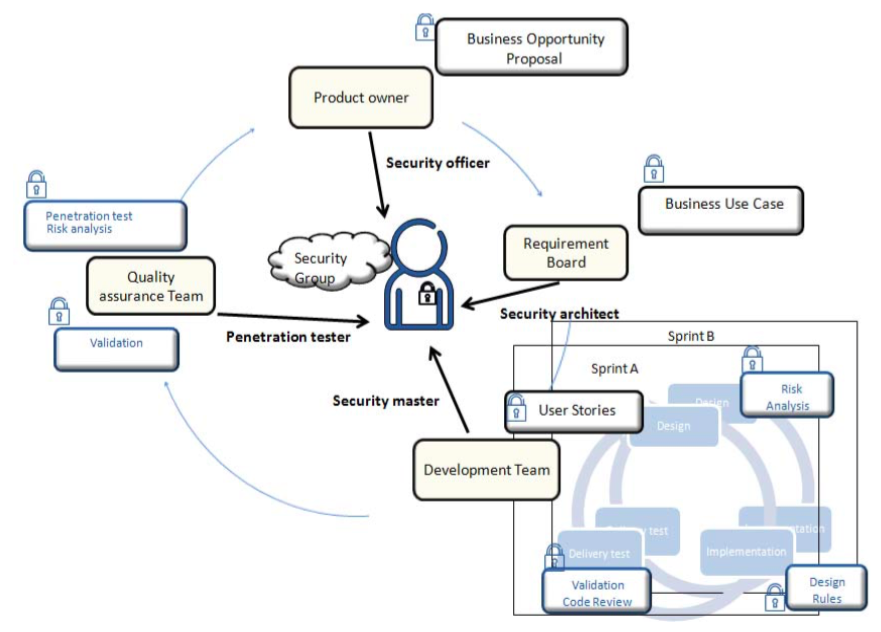
\includegraphics[width=\textwidth]{img/seapmodell.png}
  \caption{SEAP. Schlösser bedeuten sicherheitsrelevante Betrachtungen. \parencite[][S. 14]{Baca:2015aa}}
  \label{fig:seapmodell}
\end{figure}

SEAP löst dieses Problem, indem es sicherheitsrelevante Betrachtungen enger an die agilen Teilprozesse bindet (vgl. \autoref{fig:seapmodell}).
Ein \emph{Business Oportunity Proposal (BOP)} ist die Beschreibung von neuer Funktionalität.
Dieser wiederum besteht aus mehreren \emph{Business Use Cases (BUC)}, welche die Anforderungen zur Erfüllung des BOP beschreiben.
Aus den BUCs werden dann feingranulare User Storys generiert.
Das Entwicklungsteam steht während der Implementierung stets in enger Verbindung mit der Security Group, die eine Risikoanalyse durchführt und entsprechend dem potentiellen Risiko angemessene Sicherheitsvorkehrungen trifft.
Während in normalen agilen Vorgehensmodellen eine Risikoanalyse pro Hauptrelease erfolgt, findet bei SEAP diese pro BUC statt.
Dadurch wird eine inkrementelle Risikoanalyse erreicht, die sich besser in den agilen Kontext fügt.
\parencite[Vgl.][S. 15]{Baca:2015aa}

Die Security Group ist dabei integraler Bestandteil der agilen Entwicklung und kann die Auslieferung eines Inkrements bei Problemen mit der Sicherheit stoppen oder verzögern. 
Durch die enge Integration in das Entwicklungsteam steht den Entwicklern jederzeit ein kompetenter Ansprechpartner für Sicherheitsfragen zur Verfügung.
Des Weiteren kann jederzeit auf neue Sicherheitsanforderungen reagiert werden.
\parencite[Vgl.][S. 15]{Baca:2015aa}

Mit einem Fokus auf kosteneffiziente Prozesse und Tools integriert SEAP sicherheitsrelevante Überlegungen in agile Vorgehensmodelle.
\parencite[][]{Baca:2015aa} untersucht die Einführung von SEAP bei Ericsson AB in einem Geldtransfersystem und evaluiert die Ergebnisse.
Ericsson benutzte zuvor ein martkgetriebenes Entwicklungsmodell, bei dem die Requirements von einer Vielzahl an Kunden gesammelt werden.
Des Weiteren bestehen die Anforderungen an das Geldtransfersystem in einem sehr hohen Sicherheitsanspruch und einer länderspezifischen Anpassung.

Nach der Einführung von SEAP konnten bei Ericsson mehrere Verbesserungen gemessen wurden.
So verbesserte sich die Anzahl der erkannten, schweren Risiken deutlich. 
Das heißt, die Grundvoraussetzung, das Erkennen von Risiken, wurde alleine durch SEAP signifikant verbessert.
Darauf aufbauend wurde analysiert, wie viele der erkannten Risiken verhindert wurden.
Die Anzahl der beseitigten Risiken wurde um 54 \% erhöht.
Außerdem konnte die Anzahl der Risiken, die auf die nächste Version verschoben wurden, um 27 \% verringert werden.
Zusätzlich wurde eine Reduktion der Anzahl der nicht beseitigen Risiken um 29 \% erreicht.
Trotz dieser Verbesserungen konnte eine Verringerung der Mannstunden zur Beseitigung eines Risiko um 45 \% auf 1,48 h erreicht werden.
Außerdem wurde der Prozess der Identifizierung der Risiken verbessert werden, so dass nur noch ca. 1,7 h anstatt 21,6 h Mannstunden zur Identifizierung eines Risikos nötig sind.
\parencite[Vgl.][S. 17 f.]{Baca:2015aa}

\subsection{Abuser Storys} 

\parencite[][]{peeters2005agile} stellt einige Erweiterungen für das Requirements Engineering in agilen Prozessen vor.
So werden die User Storys um sogenannte \emph{Abuser Stories} ergänzt.
Eine Abuser Story ähnelt formal einer User Story, beschreibt jedoch wie ein Angreifer das System missbrauchen kann, um an Daten o. ä. zu kommen.
Gegenüber einer User Story wird eine Abuser Story nicht über den Wertbeitrag priorisiert, sondern über das potentielle Risiko und den Schaden durch den Angriff.
Dabei wird einerseits der potentielle Schaden, andererseits die Eintrittswahrscheinlichkeit zur Berechnung herangezogen.
Eine Abuser Story sollte, bei Bezug zu einer User Story, Kosten (Schäden) in gleicher Höhe wie der Wertbeitrag der User Story besitzen:
$$Wertbeitrag(UserStory) - Schaden(AbuserStory) = 0$$
Dadurch kann die Abuser Story als Umkehrfunktion betrachtet werden, die den Wertbeitrag der User Story wieder vernichtet, wenn das Szenario eintritt (vgl. \autoref{fig:abuser-story}).

\begin{figure}
  \centering
  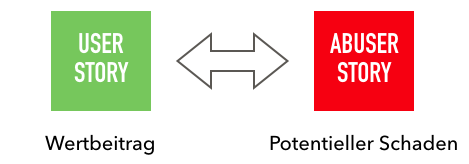
\includegraphics[width=0.6 \textwidth]{img/abuser-story.png}
  \caption{Verhältnis zwischen User und Abuser Story}
  \label{fig:abuser-story}
\end{figure}

Die Aufwandsschätzung einer Abuser Story bezieht sich dabei auf den Aufwand, der nötig ist, um das System gegen den Angriff zu schützen.
Eine \emph{Widerlegung} ist das Gegenstück zu einem Test. 
Sie zeigt, dass durch die getroffenen Gegenmaßnahmen der Angriff nicht mehr möglich ist bzw. die Wahrscheinlichkeit auf ein erträgliches Maß reduziert wurde.
\parencite[Vgl.][S. 2]{peeters2005agile}

Diese Ergänzung des agilen Modells stellt eine einfache Art dar, die Requirements Engineering Phase durch Sicherheitsbetrachtungen zu ergänzen, ohne die grundlegenden agilen Abläufe maßgeblich zu verändern.

\subsection{Kompatibilität mit Normen} % 1 Seite

\parencite[][]{Theunissen:2003:SAS:954014.954034} verweist darauf, dass agile Vorgehensmodelle durchaus die Norm ISO 12207 erfüllen können.
Es wird erkannt, dass es wichtig ist, trotz Erfüllung der Norm die Kernaussagen der agilen Methoden (Software anstatt übermäßiger Dokumentation) nicht aus den Augen zu verlieren.
Dies soll nicht bedeuten, auf Dokumentation komplett zu verzichten, sondern lediglich den Fokus auf die Softwareentwicklung zu legen und nur in den Bereichen, in denen es erforderlich ist, die nötige Dokumentation zu erzeugen.
Beispielsweise kann dies als eine Anforderung ausgedrückt werden und somit in die Systemspezifikation integriert werden.
Hier bietet sich auch ein Optimierungspotential, in dem Dokumentation, wo möglich, automatisiert generiert wird.
Dabei sollte jedoch als ultimative Quelle der Quellcode dienen, denn dieser stellt die exakteste \enquote{Dokumentation} dar.
Möglicherweise müssen dann gewissen Code-Standards definiert und implementiert werden.

Auf der Norm ISO 12207 aufbauend ist auch die Norm der ECSS grundsätzlich kompatibel zu agilen Methoden.
Eine Fallstudie bei der Swedish Space Corporation (SSC) untermauert diese Aussage \parencite[vgl.][S. 1]{Ahmad:2010:ESC:1890810.1890816}.
Durch die Norm wird dem Lieferanten keine Vorgehensmodell vorgeschrieben.
Die starke Kollaboration zwischen Lieferant und Kunde passt sehr gut zu den agilen Methoden.
Kunden definieren funktionale und nicht-funktionale (Leistungs-) Anforderungen für den Lieferanten.
Das rekursive Kunden-Lieferanten-Konzept lässt sich mit Scrum abbilden und die einzelnen Prozesse, die in der Norm definiert sind können durch agile Methoden abgebildet werden (vgl. \autoref{tab:ecss_mapping}).

\begin{table}[h]
\center
\caption{ECSS Prozesse und agile Methoden bei SSC \parencite[in Anlehnung an][S. 5]{Ahmad:2010:ESC:1890810.1890816}.}
\label{tab:ecss_mapping}
\begin{tabularx}{\textwidth}{p{6cm}|X}
ECSS Prozess & agile Methode\\
\hline
\hline
Software Management Process & Entwicklung eines Softwareentwicklungsplans, der Scrum für jedes Projekt vorschreibt.\\
\hline
Software Engineering Process & Sprintplanung bei Beginn des Sprints und testgetriebene Entwicklung als Entwicklungsmethode.\\
\hline
Software Verification and Validation Process & Häufige Review-Meetings in Scrum und testgetrieben Entwicklung stellen die Prozessverifikation sicher und minimieren Probleme.\\
\hline
Assurance Program Implementation & Sprintplanungs-Meeting, tägliche Meetings und die Retrospektive helfen bei der Implementierung.\\
\hline
Software Process Assurance & Durch tägliche Meetings und häufige Retrospektiven.\\
\hline
Software Product Quality Assurance & Häufige Retrospektiven identifizieren Erfolgsfaktoren und Fehlschläge.\\
\end{tabularx}
\end{table}

Schließlich sollte die Norm ständig aktuell gehalten werden, um auf geänderte Anforderungen der Industrie und die tatsächlich gelebte Praxis zu reagieren.
ECSS ist sehr flexibel und lässt viele Freiheiten, sofern die Qualität hoch ist und gewisse Anforderungen im Vorgehensmodell eingehalten werden.
\parencite[Vgl.][S. 6]{Ahmad:2010:ESC:1890810.1890816}




























